\documentclass{beamer}
\usepackage{preamble_beamer}
\usepackage{comment}


\title[Случайные процессы]{Лекция 1. Теория вероятностей. Случайные процессы с дискретным временем} % The short title appears at the bottom of every slide, the full title is only on the title page


\begin{document}

\begin{frame}
\titlepage 
\end{frame}
%\begin{comment}

\begin{frame}{План}
    \begin{itemize}
        \item Вероятностное пространство: определения и свойства
        \item Условное математическое ожидание
        \item Фильтрация: определение и свойства
        \item Случайные процессы: основные опредлеения
        \item Мартингалы, моменты остановки
        \item Теоремы Дуба. Дискретный стохастический интеграл
    \end{itemize}
\end{frame}

% введение: теорвер
\begin{frame}{Вероятностное пространство}
    \begin{block}{Определение}
        Вероятностное пространство это тройка $(\Omega, \F, \PP)$, где:
        \begin{itemize}
            \item $\Omega$ -- пространство элементарных исходов,
            \item $\F \subseteq 2^{\Omega}$ -- $\sigma$-алгебра событий,
            \item $\PP$ -- счётно-аддитивная вероятностная мера.
        \end{itemize}
    \end{block}    
\end{frame}

\begin{frame}{$\sigma$-алгебра}
    \begin{block}{Определение}
        Пусть $\Omega$ -- множество. Семейство подмножеств $\Omega$ $\F$ называется алгеброй, если:
        \begin{itemize}
            \item $\emptyset \in \F$
            \item $\forall A, B \in \F$: $A\cup B\in \F$
            \item $\forall A \in \F$: $\Omega\backslash A \in \F$
        \end{itemize}
    \end{block}
    Алгебра $\F$ называется $\sigma$-алгеброй, если она замкнута относительно счётного объединения: 
    $$\forall A_1, A_2, \ldots \in \F: \bigcup_{n=1}^{\infty} A_n \in \F$$

    Примеры:
    \begin{itemize}
        \item $\F=(\emptyset, \Omega)$ -- тривиальная $\sigma$-алгебра
        \item $\F=2^{\Omega}$ -- множество всех подмножеств
        \item $\Omega = \{1,2,3,4\}$, $\F=\{ \emptyset, \Omega, \{1, 2\}, \{3, 4\} \}$
    \end{itemize}
\end{frame}

\begin{frame}{$\sigma$-алгебра}
    Пусть $\Omega$ -- множество, $\F$ -- $\sigma$-алгебра. Тогда:
    \begin{itemize}
        \item $\emptyset \in \F, \Omega \in \F$
        \item $\forall A, B \in \F: A\cap B\in \F$
        \item $\forall A_1, A_2, \ldots \in \F: \bigcap_{n=1}^{\infty} A_n \in \F$
        \item Если $G$ -- $\sigma$-алгебра, то $\F\cap G$ -- $\sigma$-алгебра
        \item Если $\{\F_{\gamma}, \gamma\in\Gamma\}$ -- семейство $\sigma$-алгебр, то $\bigcap_{\gamma \in \Gamma} \F_{\gamma}$ -- $\sigma$-алгебра.
    \end{itemize}
    \begin{block}{Определение}
        Пусть $\Omega=\mathbb{R}$. Борелевская $\sigma$-алгебра $B(\mathbb{R})$ -- минимальная сигма-алгебра, содержащая все множества вида $(-\infty, a)$, $a\in \mathbb{R}$.
    \end{block}

    По определению $\sigma$-алгебры, борелевская $\sigma$-алгебра содержит также все отрезки, лучи, интервалы и полуинтервалы, открытые и закрытые множества.
\end{frame}

\begin{frame}{Вероятностная мера}
    \begin{block}{Определение}
        Вероятностная мера $\PP$ это неотрицательная функция на $\F$, удовлетворяющая свойствам:
        \begin{itemize}
            \item $\PP(\emptyset) = 0$
            \item $\PP(\Omega) = 1$
            \item $\forall A_1, A_2, \ldots \in \F: \PP\left(\bigsqcup_{n=1}^{\infty}A_n\right) = \sum_{n=1}^{\infty} \PP(A_n)$ 
        \end{itemize}
    \end{block}
    Пример. Пусть $\Omega = \{1, 2, \ldots, n\}$, $\F=2^{\Omega}$. Тогда $\PP(A)=\dfrac{\#A}{n}$ -- вероятностная мера.
\end{frame}

\begin{frame}{Случайные величины}
    Пусть $(\Omega, \mathcal{\F}, \PP)$ -- вероятностное пространство. 
    \begin{block}{Определение}
        Функция $\xi(\omega): \Omega \to \mathbb{R}$ называется измеримой относительно $\sigma$-алгебры ${\F}$, если $\forall x \in \mathbb{R}$:
        $$
            \{\omega : \xi(\omega) < x \} \in {\F}
        $$
    \end{block}
    Измеримые функции также будем называть случайными величинами (коротко с.в.). Обозначение $\xi \in \mathcal{\F}$.
    Множество $\{\omega : \xi(\omega) < x \}$ также будем записывать как $\{ \xi < x\}$.

    \begin{block}{Утверждение}
    Если $\xi \in \mathcal{\F}$, то:
        \begin{itemize}
            \item $\{\xi \geq x \} \in {\F}$
            \item $\{y \leq \xi < x \} \in {\F}$
            \item $\{\xi = x \} \in {\F}$
        \end{itemize}
    \end{block}
\end{frame}

\begin{frame}{Случайные величины}
    \begin{block}{Определение}
        Пусть $\xi : \Omega\to\mathbb{R}$ -- функция.
        Положим 
        $$\sigma(\xi) = \{ \xi^{-1}(A), A\in \mathcal{B}(\mathbb{R})\}$$
    \end{block}
    \begin{block}{Утверждение}
         $\sigma(\xi)$ -- минимальная $\sigma$-алгебра, относительно которой $\xi$ измерима.
    \end{block}
\end{frame}

\begin{frame}{Случайные величины и мера}
    \begin{block}{Определение}
        Функция распределения $F: \R\to[0, 1]$ с.в. $\xi$ называется функция:
        $$
            F = \PP(\xi < x).
        $$Определение корректно, так как $\{\xi < x\} \in \F$
    \end{block}
    \begin{block}{Определение}
        Распределением $\mu_{\xi}$ с.в. $\xi$ называется вероятностная мера на $\left(\R, \mathcal{B}(\R)\right)$, определённая как:
        $$
            \mu_{\xi}(B) = \PP(\xi \in B) = \PP(\xi^{-1}\left( B \right))\;\forall B\in\mathcal{B}(\R)
        $$
    \end{block}
    Случайные величины переносят меру $\PP$ c $(\Omega, \F)$ на $(\R, \mathcal{B}(\R))$. 
\end{frame}

\begin{frame}{Мат. ожидание} 
    \begin{block}{Определение}
    Мат. ожидание $\E \xi$ с.в. $\xi$ это интеграл Лебега по $\Omega$:
        $$
            \E \xi = \int_{\Omega}\xi(\omega)d\PP(\omega)
        $$
    \end{block}
    \begin{block}{Утверждение}
        Для произвольной функции $g : \R \to \R$ такой, что $g(\xi)$ интегрируема выполнено:
        $$
            \E g(\xi) = \int_{\Omega} g(\xi(\omega))d\PP(\omega)=\int_{\R} g(x) d\mu_{\xi}(x) = 
            \int_{\R} g(x) dF(x)
        $$
        Если $\mu_{\xi}$ имеет плотность $p_{\xi}(x)$, то:
        $$
            \E g(\xi) = \int_{\R} g(x) p_{\xi}(x) dx
        $$
    \end{block}
\end{frame}

\begin{frame}{Сигма-алгебры и разбиения}
    Пусть $\Omega$ -- пространство элементарных исходов.
    
    Пусть $\mathcal{A} = \{A_i\}_{i=1}^n$ -- разбиение множества $\Omega$, т.е.:
    $$\bigcup_i A_i = \Omega, \; A_i \cap A_j = \emptyset$$

    \begin{center}
        
\includegraphics[width=0.25\textwidth]{8_figs/разбиение.png}
    \end{center}

    $\mathcal{H} = \sigma(\mathcal{A})$ -- $\sigma$-алгебра, порождённая разбиением. Состоит из элементов вида 
    $B = \bigcup_{k} A_{n_k}$.
\end{frame}

\begin{frame}{Сигма-алгебры и случайные величины}
    \begin{block}{Теорема}
        Пусть $(\Omega, \mathcal{F} , P)$ -- вероятностное пространство. Пусть $\xi: \Omega \to \R$ -- принимает конечное число значений $\{a_1, \ldots, a_n\}$.
        Пусть $A_i = \xi^{-1}(a_i)$. Тогда $\xi(\omega)$ измерима $\Longleftrightarrow \forall i \; A_i \in \mathcal{F}$
    \end{block}
    \textit{Доказательство.}
    $\{ \xi < x \} = \bigcup\limits_{a_i < x} \{ \xi = a_i\} = \bigcup\limits_{a_i < x} A_i$.
\end{frame}

% условное мат. ожидание
\begin{frame}{УМО}
    Пусть $\left( \Omega, \mathcal{F} , \PP\right)$ -- вероятностное пространство. Пусть $A, B \in \mathcal{F} $, $\PP(B) \neq 0$. 
    \begin{block}{Определение}
        Условная вероятность: 
        $$
            \PP(A|B) = \dfrac{\PP(A\cap B)}{\PP(B)}
        $$
    \end{block}

    \begin{block}{Определение}
        Пусть $\xi \in \mathcal{F}$. Условным мат. ожиданием $\xi$ при условии $B$ будем называть число:
        $$\mathbb{E}^B \xi = \dfrac{\mathbb{E} \left(\xi \mathbb{I}_{B}\right)}{\PP(B)}$$
    \end{block}
    Также будем использовать обозначение $\mathbb{E}\left[ \xi | B \right]$
\end{frame}

\begin{frame}{УМО для дискретной $\sigma$-алгебры}
    Пусть $\mathcal{A} = \{A_i\}_{i=1}^n$ -- разбиение множества $\Omega$, $\mathcal{H} = \sigma(\mathcal{A})$ -- $\sigma$-алгебра, порождённая этим разбиением.

    \begin{block}{Определение}
        Пусть $\xi \in \mathcal{F}$. Условным мат. ожиданием $\xi$ при условии $\mathcal{H}$ будем называть случайную величину:
        $$\mathbb{E}\left[ \xi | \mathcal{H} \right] = \sum_{i=1}^n \mathbb{I}_{A_i} \dfrac{\mathbb{E} \left(\xi \mathbb{I}_{A_i}\right)}{P(A_i)} = 
        \sum_{i=1}^n \mathbb{I}_{A_i} \mathbb{E}^{A_i}\xi$$
    \end{block}

    $\mathbb{E}\left[ \xi | \mathcal{H} \right]$ -- дискретная случайная величина:
    $$
        \mathbb{E}\left[ \xi | \mathcal{H} \right](\omega) = \mathbb{E}^{A_i} \xi, \text{если } \omega \in A_i
    $$
\end{frame}

\begin{frame}{УМО для дискретной $\sigma$-алгебры}
    \begin{block}{Задача}
        Пусть $\xi \sim N(0, 1)$, $\mathcal{H} = \sigma\left( \{\xi \geq 0\}, \{\xi < 0\} \right)$. Найти $\E \left[ \xi | \mathcal{H} \right]$
    \end{block}
    \textit{Решение}. Пусть $A_1 = \{\xi \geq 0\}, A_2 = \{\xi < 0\}$. Тогда:
    $$
        \E^{A_1} \xi = \dfrac{\E \xi \mathbb{I} (\xi \geq 0)}{\PP(A_1)} = 2 \cdot \int_0^{\infty} x p_{\xi}(x) dx = 2 \cdot \dfrac{1}{\sqrt{2\pi}} \int_0^{\infty} x e^{-0.5x^2} dx
        = \sqrt{\dfrac{2}{\pi}}
    $$
    Аналогично:
    $$
        \E^{A_2} \xi = -\sqrt{\dfrac{2}{\pi}}
    $$
    Откуда:
    $$
        \E \left[ \xi | \mathcal{H} \right] = \sqrt{\dfrac{2}{\pi}} \cdot \mathbb{I}(\xi \geq 0) -\sqrt{\dfrac{2}{\pi}} \cdot \mathbb{I}(\xi < 0)
        = \sqrt{\dfrac{2}{\pi}} \cdot \mathrm{sgn}(\xi)
    $$где
    $$
        \mathrm{sgn}(\xi) = \begin{cases}
            1, \xi \geq 0 \\
            -1, \xi < 0
        \end{cases}
    $$
\end{frame}

\begin{frame}{УМО: свойства}
    Пусть $\mathcal{A} = \{A_i\}_{i=1}^n$ -- разбиение, $\mathcal{H} = \sigma(\mathcal{A})$. Пусть $\eta = \mathbb{E}\left[ \xi | \mathcal{H} \right]$. Тогда:
    \begin{itemize}
        \item $\eta \in \mathcal{H}$
        \item $\forall A\in \mathcal{H}$:
        $$
            \mathbb{E} \left[ \eta \cdot \I_{A} \right] = \mathbb{E} \left[ \xi \cdot \I_A \right]
        $$
    \end{itemize}
    Первое утверждение очевидно, второе достаточно проверить для $A\in \mathcal{A}$.
\end{frame}

\begin{frame}{УМО для произвольной $\sigma$-алгебры}
    \begin{block}{Определение}
        Пусть $(\Omega, \F, \PP)$ -- вероятностное пространство, пусть $\xi$ -- интегрируемая с.в. Пусть $\mathcal{H} \subseteq \F$ -- $\sigma$-алгебра. Тогда с.в. $\eta$, удовлетворяющая свойствам:
    \begin{itemize}
        \item $\eta \in \mathcal{H}$
        \item $\forall A\in \mathcal{H}$:
        $$
            \mathbb{E} \left[ \eta \cdot \I_{A} \right] = \mathbb{E} \left[ \xi \cdot \I_A \right]
        $$
    \end{itemize} называется условным мат. ожиданием $\xi$ при условии $\mathcal{H}$ и обозначается:
    $$
        \eta = \mathbb{E}\left[ \xi | \mathcal{H} \right]
    $$
    \end{block}
    \textit{Замечание} 
    В отличии от предыдущего определения $\mathcal{H}$ -- произвольная $\sigma$-подалгебра. Можно доказать, что такая с.в. $\eta$ всегда существует и п.н. единственна.
\end{frame}

\begin{frame}{УМО: свойства}
    \begin{itemize}
        \item Линейность
        $$
            \mathbb{E}\left[ \alpha \xi + \beta \eta | \mathcal{H} \right]
            = \alpha \mathbb{E}\left[ \xi  | \mathcal{H} \right] + \beta \mathbb{E} \left[ \eta  | \mathcal{H} \right]
        $$

        \item Если $\xi \in \mathcal{H}$, то $\mathbb{E}\left[ \xi | \mathcal{H} \right] = \xi$

        \item Если $\xi \perp \mathcal{H}$, то $\mathbb{E}\left[ \xi | \mathcal{H} \right] = \mathbb{E} \xi$
        
        \item Повторное мат. ожидание. Пусть $\mathcal{G}$ -- $\sigma$-подалгебра $\mathcal{H}$. 
        $$
            \mathbb{E} \left[ \mathbb{E}\left[ \xi | \mathcal{H} \right] | \mathcal{G} \right] = \mathbb{E}\left[ \xi | \mathcal{G} \right]
        $$
        В частности:
        $$
            \mathbb{E} \xi = \mathbb{E} (\mathbb{E}\left[ \xi | \mathcal{H} \right]) 
        $$

        \item Неравенство Йенсена. Если $f$ выпуклая, то:
        $$
            f(\mathbb{E}\left[ \xi | \mathcal{H} \right]) \leq \mathbb{E}\left[ f(\xi) | \mathcal{H} \right]
        $$

        \item Если $\eta \in \mathcal{H}$, то
        $$
            \mathbb{E} \left[ \eta\cdot\xi | \mathcal{H} \right] = \eta \cdot \mathbb{E}\left[ \xi | \mathcal{H} \right] 
        $$
    \end{itemize}
\end{frame}

\begin{frame}{УМО как проекция}
    \begin{block}{Утверждение}
        Пусть $\xi$ -- квадратично-интегрируемая с.в., т.е. $\mathbb{E} \xi^2 < \infty$. Пусть $\mathcal{H}$ -- $\sigma$-подалгебра $\F$. Тогда:
        $$
            \mathbb{E}\left[ \xi | \mathcal{H} \right] = \arg \min_{z \in \mathcal{H}} \E (\xi-z)^2
        $$
    \end{block}
    \pause

    Пусть $\xi, \eta$ -- случайные величины. Положим:
    $$
        \E\left[\xi | \eta\right] = \mathbb{E}\left[ \xi | \sigma(\eta) \right]
    $$

    Так как $\E\left[\xi | \eta\right] \in \sigma(\eta)$, то $\exists g:\R\to\R$: 
    $$
        \E\left[\xi | \eta\right] = g(\eta)
    $$
    \pause
    \begin{block}{Утверждение}
    $$
        \mathbb{E}\left[ \xi | \eta \right] = \arg \min_{g \in \R \to \R} \E (\xi-g(\eta))^2
    $$
    \end{block}
\end{frame}

\begin{frame}{УМО относительно случайной величины}


    \begin{block}{Задача}
        Пусть $\xi, \eta$ -- i.i.d. Найти $\E \left[ \xi | \xi + \eta\right]$.
    \end{block}
    \textit{Решение}. 
    
    Пусть $\alpha = \E \left[ \xi | \xi + \eta\right]$. В силу симметрии $$\E \left[ \xi | \xi + \eta\right] = \E \left[ \eta | \xi + \eta\right]$$
    Складываем левую и правую часть, получим: $$2\alpha =\E \left[ \xi + \eta | \xi + \eta\right] = \xi + \eta$$
    Откуда
    $$
        \E \left[ \xi | \xi + \eta\right] = \E \left[ \eta | \xi + \eta\right] = \dfrac{\xi+\eta}{2}
    $$

    \begin{block}{Задача}
        Пусть $X, Y$ имеют совместное нормальное распределение с параметрами $\mu = (\mu_X, \mu_Y), \Sigma = \begin{pmatrix}
            \sigma_X^2 & \sigma_{XY} \\
            \sigma_{XY} & \sigma_Y^2
        \end{pmatrix}$. Найти $\E \left[ X | Y\right]$
    \end{block}
\end{frame}
% % производная Радона-Никодима
% \begin{frame}{Абсолютная непрерывность мер}
%     Пусть $(\Omega, \F)$ -- измеримое пространство (множество с $\sigma$-алгеброй). Пусть $\Q, \PP$ -- меры на $(\Omega, \F)$.

%     \begin{block}{Определение}
%         Мера $\Q$ абсолютно непрерывна относительно $\PP$, если $\forall A \in \F$:
%         $$
%             \PP(A) = 0 \to \Q(A) = 0
%         $$Обозначение $\Q \ll \PP$
%     \end{block}

%     \begin{block}{Определение}
%         Мера $\Q$ эквивалентна $\PP$, если $\Q \ll \PP, \PP \ll \Q$. Обозначение $\Q \sim \PP$
%     \end{block}
% \end{frame}

% \begin{frame}{Абсолютная непрерывность мер: примеры}
%     Примеры:
%     \begin{itemize}
%         \item     Пусть $\Omega = \mathbb{N}, \F=2^{\mathbb{N}}$. Тогда:
%     $$
%         \Q \ll \PP \Leftrightarrow \PP(\{n\}) = 0 \to \Q(\{n\}) = 0
%     $$

% \item     Пусть $\Omega=\R, \F = \mathcal{B}(\R)$. Пусть $$\PP(dx) = p(x)dx, \Q(dx) = q(x) dx.$$

% Тогда 
%     $$
%         \Q \ll \PP \Leftrightarrow \mathrm{supp}(p) \subseteq\mathrm{supp}(q)
%     $$
%     где 
%     $$
%         \mathrm{supp}(f) = \{x \in \R : f(x) \neq 0 \}
%     $$
%     \end{itemize}
% \end{frame}

% \begin{frame}{Абсолютная непрерывность мер: примеры}
%     Пусть $\Omega=\R, \F = \mathcal{B}(\R)$

%     Пусть $d\PP(x)= \mathbb{I}(x \in [-1, 1]) dx$, $d\Q(x) = \mathbb{I}(x \in [0, 1]) dx$.

%     \begin{itemize}
%         \item Верно ли, что $\Q \ll \PP$?
%         \item Верно ли, что $\Q \sim \PP$?
%     \end{itemize}
% \end{frame}

% \begin{frame}{Производная Радона-Никодима}
%     Пусть $\PP$ -- мера, $f \in \F$ -- фунцкия, $f(\omega)\geq 0$. Определим меру $\Q$ по формуле:
%     $$
%         \Q(A) = \int_A f(\omega) d\PP(\omega), \; A \in \F
%     $$
    
%     Тогда $\Q$ -- мера и $\Q \ll \PP$. 
    
%     Верно и обратное:
%     \begin{block}{Теорема Радона-Никодима}
%         Пусть $\Q \ll \PP$. Тогда $\exists f \in \F, f(\omega) \geq 0$:
%         $$
%             \Q(A) = \int_A f(\omega) d\PP(\omega)
%         $$Обозначение: $f(\omega) = \dfrac{d\Q}{d\PP}$
%     \end{block}
% \end{frame}

% \begin{frame}{Производная Радона-Никодима: примеры}
%     \begin{itemize}
%         \item     Пусть $\Omega = \mathbb{N}, \F=2^{\mathbb{N}}$, $\Q \ll \PP$.
%         Тогда:
%     $$
%          \dfrac{d\Q}{d\PP}(n) = \dfrac{\Q(\{n\})}{\PP(\{n\})} \cdot \mathbb{I}(\PP(\{n\}) \neq 0)
%     $$при $n \in \mathbb{N}$.

% \item     Пусть $\Omega=\R, \F = \mathcal{B}(\R)$. Пусть 
%     $$\PP(dx) = p(x)dx, \Q(dx) = q(x) dx$$ и $\Q \ll \PP$. Тогда:
%     $$
%         \dfrac{d\Q}{d\PP}(x) = \dfrac{q(x)}{p(x)} \cdot \mathbb{I}(p(x) \neq 0)
%     $$
%     \end{itemize}
% \end{frame}

% \begin{frame}{Производная Радона-Никодима: свойства}
%     Пусть 
%     \begin{itemize} 
%         \item $(\Omega, \F)$ -- измеримое пространство
%         \item $\PP \sim \Q$ -- вероятностные меры
%         \item $f=\dfrac{d\Q}{d\PP}$ -- производная Радона-Никодима 
%         \item $\xi \in \F$ -- случайная величина.
%     \end{itemize}
%     Тогда:
%     \begin{itemize}
%         \item $Q(A) = \int_{A} f(\omega) d\PP(\omega)$
%         \item $\E^{\Q} \xi = \int_{\Omega} \xi(\omega) dQ(\omega) = \int_{\Omega} \xi(\omega) f(\omega) d\PP(\omega)
%         = \E^{\PP} \left[\xi \cdot f\right]$ 
%         \item $\E^{\Q} 1 = \E^{\PP} f = 1$
%     \end{itemize}

%     \begin{block}{Задача}
%         Пусть $\xi \sim N(0, 1)$, $p_{\xi}(x) = \frac{1}{\sqrt{2\pi}}e^{-0.5x^2}$. 
%         \begin{itemize}
%             \item Найти меру (плотность) относительно которой $\xi \sim N(a, 1)$.
%             \item Найти производную Радона-Никодима $f$.
%             \item Убедиться, что $\Ef = 1, \; \E [f\cdot \xi] = a$.
%         \end{itemize}
%     \end{block}
% \end{frame}
% случайные процессы
\begin{frame}{Случайные процессы}
\begin{block}{Определение}
    Пусть $(\Omega, \F, \PP)$ -- вероятностное пространство. Пусть $\mathcal{T}$ -- некоторое множество индексов. Случайным процессом $\xi$ будем называть совокупность с.в. $\{\xi_t\}_{t\in \mathcal{T}}$, заданных на одном вероятностном пространстве.
\end{block}
\begin{itemize}
    \item Случайный процесс -- функция двух переменных: $\xi : \mathcal{T} \times \Omega \to \R$, измеримая по второму аргументу.
    \item Если $\mathcal{T}$ конечно, то случаный процесс = многомерная с.в.
    \item Обычно $\mathcal{T} \in \{ \mathbb{N}, \R^+, [0, T]\}$.
    \item Для фиксированного $t\in \mathcal{T}$ отображение 
    $\omega \mapsto\xi(t, \omega)$  которое обозначим $\xi_t$ -- сечение процесса $\xi$.
    \item Для фиксированного $\omega$ отображение $t \mapsto \xi(t, \omega)$ -- детерменированная функция, реализация(траектория) случайного процесса.
\end{itemize}
\end{frame}

\begin{frame}{Случайные процессы}
    \begin{block}{Конечномерные распределения}
    Всевозможные совместные распределения с.в. $\xi_{t_1}, \ldots, \xi_{t_n}$ называются конечномерными распределениями процесса $\xi_t$:
    $$
        F_{t_1, \ldots, t_n} (x_1, \ldots, x_n) = \PP(\xi_{t_1} \leq x_1, \ldots, \xi_{t_n} \leq x_n)
    $$
\end{block}
\begin{itemize}
    \item Мат. ожидание случайного процесса: $m(t)=\mathbb{E} \xi_t$
    \item Автоковариационная функция: $b(t, s) = \mathrm{cov}(\xi_t, \xi_s)$
\end{itemize}
\end{frame}

\begin{frame}{Случайные процессы: пример}
    
    \textit{Примеры.}
    \begin{itemize}
        \item $\mathcal{T}=[0,1]$. Пусть $\eta \sim N(0,1)$. Положим $\xi_t = t \cdot \eta$.
    \end{itemize}
    Свойства:
    \begin{itemize}
        \item $\E \xi_t = 0$
        \item $\mathbb{D} \xi_t = t^2$
        \item $cov(\xi_t, \xi_s) = ts$
    \end{itemize}
    
    % \begin{figure}[ht]
    % \centering
    % 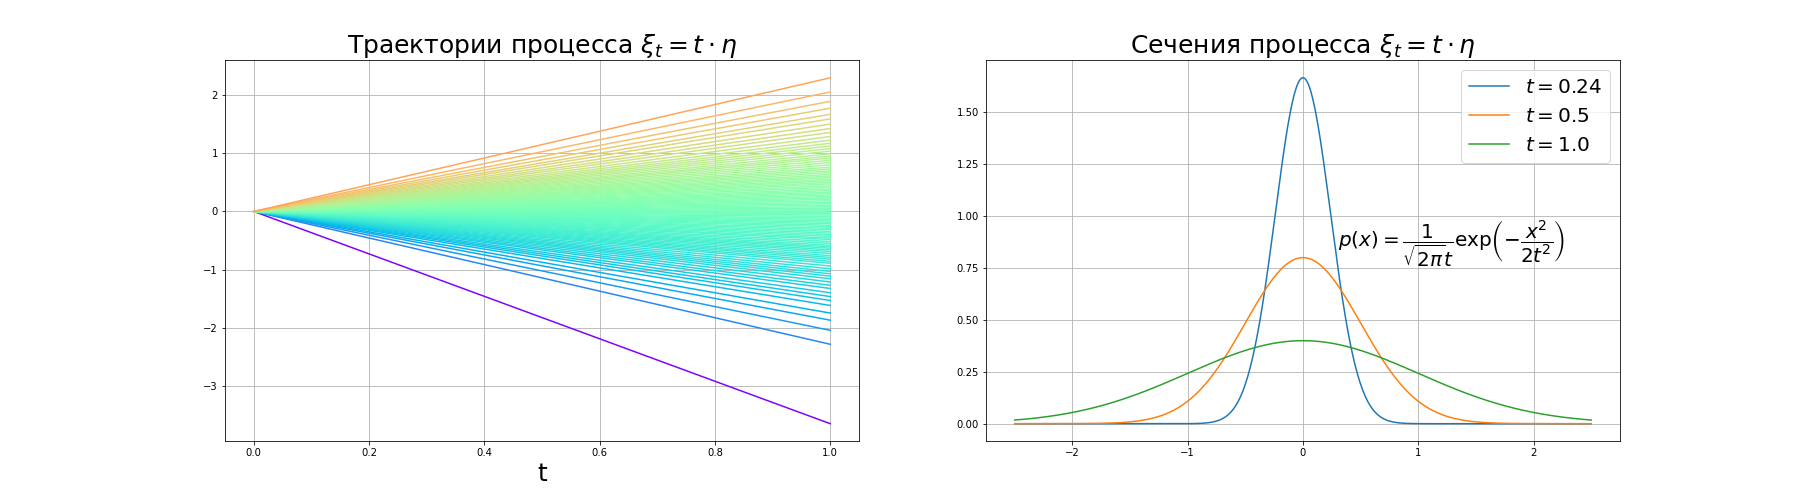
\includegraphics[width=1.2\textwidth]{1_figs/process_example_1.png}
    % \end{figure}

    \noindent\makebox[\textwidth]{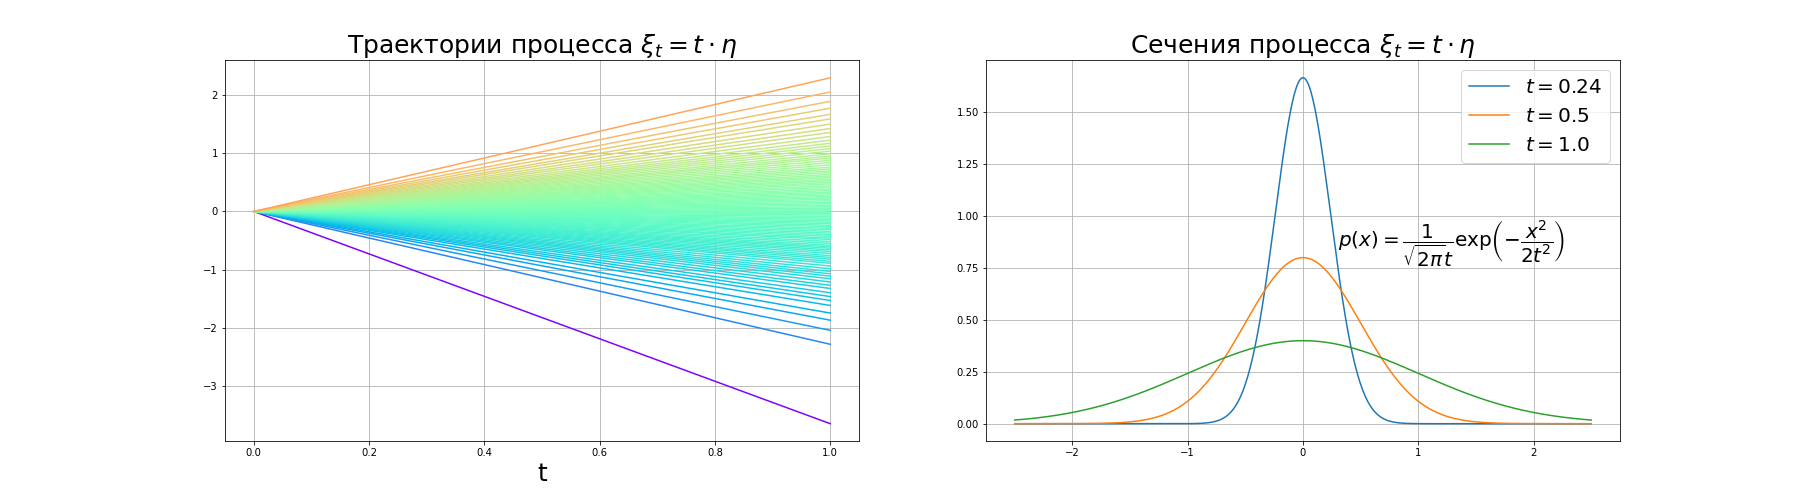
\includegraphics[width=1.2\textwidth]{1_figs/process_example_1.png}}

\end{frame}

\begin{frame}{Случайные процессы: пример}
Здесь и далее будем считать, что $\xi \sim Be(p)$ если
    $$
        \xi = \begin{cases}
            +1, \text{с вер. } p\\
            -1, \text{с вер. } 1-p
        \end{cases}
    $$
    Пусть $\mathcal{T}=\mathbb{N}$, $\xi_t \sim Be(1/2)$ -- i.i.d.
    \begin{block}{Определение}
        Простое случайное блуждание $X_t$ это случайный процесс:
        \begin{align*}
            & X_t = \sum_{s=1}^{t} \xi_s \\
            & X_0 = 0
        \end{align*}            
    \end{block}
    Свойства:
    \begin{itemize}
        \item $\mathbb{E} X_t = 0, \; \mathbb{D} X_t = t$
        \item $\mathbb{E} \left[ X_t | X_{t-1} \right] = X_{t-1}$
        \item $\mathrm{cov}(X_t, X_s) = \min(t, s)$
    \end{itemize}
\end{frame}

\begin{frame}{Случайное блуждание: траектории}
    \noindent\makebox[\textwidth]{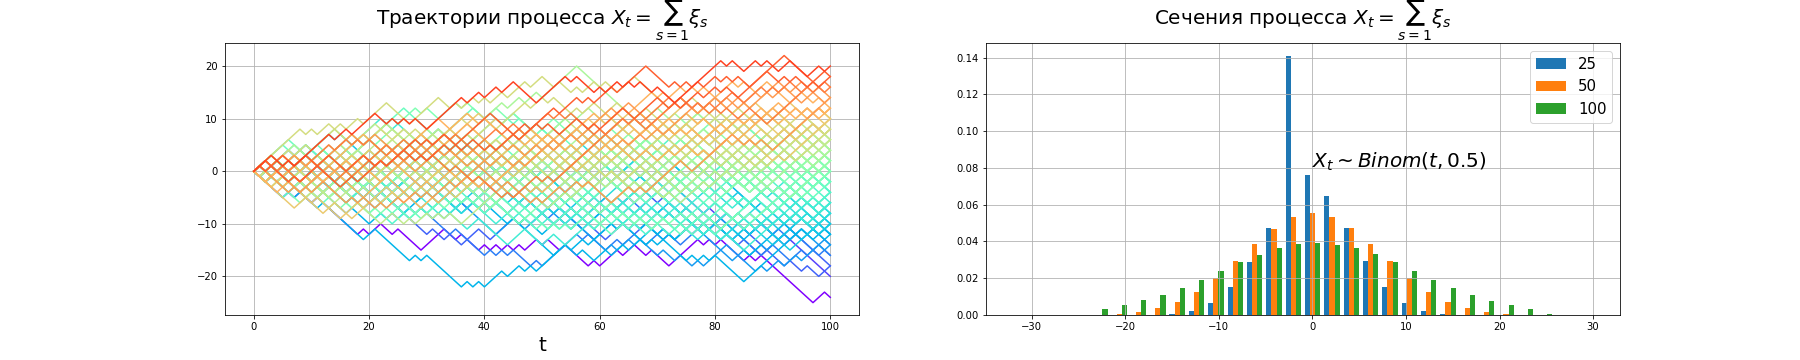
\includegraphics[width=1.2\textwidth]{1_figs/process_example_2.png}}
\end{frame}
% фильтрация
\begin{frame}{Фильтрация}
    Пусть $\mathcal{T} = \mathbb{N}$.
    \begin{block}{Определение}
        Пусть \((\Omega, \mathcal{F}, \PP)\) -- вероятностное пространство.
        
        Фильтрацией $(\mathcal{F}_t)_{t \geq 0}$ называется последовательность вложенных $\sigma$-подалгебр:
        $$
            (\mathcal{F}_t)_{t \geq 0}: \; \mathcal{F}_s \subseteq \mathcal{F}_t, \forall s\leq t
        $$
        где $\F_t \subseteq \mathcal{F}$ -- $\sigma$-под алгебры.   
    \end{block}

    $\mathcal{F}_t$ -- информация, доступная к моменту времени $t$.

    Процесс $\{\xi_t\}$ -- \textbf{адаптированный}, если $\xi_t \in \F_t \forall t \in \mathbb{N}$.

    Процесс $\{\xi_t\}$ -- \textbf{предсказуемый}, если $\xi_t \in \F_{t-1} \forall t \in \mathbb{N}$.
\end{frame}

\begin{frame}{Естественная фильтрация}
    \begin{block}{Определение}
        Пусть $\{\xi_t\}$ -- случайный процесс. Определим:
        $$
            \mathcal{F}_t = \sigma(\{\xi_s, s \leq t\}),
        $$т.е. $\mathcal{F}_t$ -- минимальная $\sigma$-алгебра, относительно которой все с.в. $\xi_s, s\leq t$ измеримы. Тогда 
        \begin{itemize}
            \item $\left(\mathcal{F}_t\right)_{t\geq 0}$ -- фильтрация
            \item $\{\xi_t\}_{t\geq 0}$ -- адаптированный к фильтрации процесс
        \end{itemize}
        $\left(\mathcal{F}_t\right)_{t\geq 0}$ называется \textbf{естественной фильтрацией}.    
    \end{block}

\end{frame}

% мартингалы
\begin{frame}{Мартингалы}
    \begin{block}{Определение}
        Пусть $(\Omega, \F, \PP)$ -- вероятностное пространство, $(\F_t)_{t\geq 0}$ -- фильтрация. Случайный процесс $(\xi_t)_{t\geq 0}$ называется \textbf{мартингалом} относительно фильтрации $(\F_t)_{t\geq 0}$, если:
        \begin{itemize}
            \item $\E |\xi_t| < \infty$ -- интегрируемость
            \item $\xi_t \in \F_t$ -- адаптированность
            \item $\E \left[ \xi_t | \F_s\right] = \xi_s$ для всех $s\leq t$ -- мартингальное свойство.
        \end{itemize}
    \end{block}
    \begin{itemize}
        \item Если фильтрация явно не указана, в качестве неё берётся естественная фильтрация процесса $(\xi_t)_{t\geq 0}$.
        \item Процесс называется суб(супер) мартингалом, если:
    $$
        \E \left[ \xi_t | \F_s\right] \geq (\leq) \xi_s
    $$
    \end{itemize}
\end{frame}

\begin{frame}{Мартингалы: примеры}
    \begin{itemize}
        \item Случайное блуждание. Пусть
        \begin{itemize}
            \item $\xi_t$ -- i.i.d., $\E \xi_t =0$,
            \item $X_t = \sum_{s=1}^{t}\xi_s$
        \end{itemize}
    Мартингальное свойство:
    $$
        \mathbb{E} \left[ X_t | \F_s\right]
        = \mathbb{E} \left[ X_t - X_s | \F_s\right]
        + \mathbb{E} \left[ X_s | \F_s\right] = X_s
    $$
    \item Геометрическое случайное блуждание. 
    \begin{itemize}
        \item $\xi_t$ -- i.i.d., $\E \xi_t = 1$, $\xi_t > 0$
        \item $X_t = \prod_{s=1}^t \xi_s$
    \end{itemize}
    Мартингальное свойство:
    $$
        \mathbb{E} \left[ X_t | \F_s\right]
        = \mathbb{E} \left[ X_s \cdot \dfrac{X_t}{X_s} | \F_s\right]
        = X_s \cdot \mathbb{E} \left[ \dfrac{X_t}{X_s} | \F_s\right] = X_s
    $$
    \end{itemize}
\end{frame}

\begin{frame}{Мартингалы: свойства}
    \begin{itemize}
        \item В дискретном случае досаточно требовать свойства:
        $$
            \E \left[ X_{t+1} | F_{t}\right] = X_t
        $$
        \item $\E X_n = \E X_0 = const$
        \item Если $(X_t)_{t\geq 0}$ -- мартингал, $f(x)$ -- выпуклая (вогнутая) функция, то процесс $\eta_t = f(X_t)$ -- суб (супер) мартингал.
        \item Мартингалы Леви: если $\eta$ -- произвольная интегрируемая случайная величина, то процесс $X_t = \E \left[ \eta|\F_t\right]$ -- мартингал. В частности, на интервале $[0, T]$ мартингал геренируется своим терминальным значением:
        $$
            X_t = \E \left[ X_T | \F_t \right]
        $$
        \item Пусть $X_t$ -- квадратично-интегрируемый мартингал, тогда его приращения некоррелированы:
        $$
            \mathrm{cov} (X_p - X_q, X_t - X_s) = 0
        $$ при $s \leq t \leq q \leq p$
    \end{itemize} 
\end{frame}

\begin{frame}{Дискретный стохастический интеграл}
    Пусть $(\Omega, \F, \PP)$ -- вероятностное пространство, $(\F_t)_{t\geq 0}$ -- дискретная фильтрация.
    \begin{block}{Определение}
    Пусть $(X_t)_{t\geq 0}, (Y_t)_{t \geq 0}$ -- случайные процессы. Будем называть процесс $Z_t$, определённый как:
    $$
        Z_t = (X\star Y)_t = \sum_{s=0}^t X_s (Y_s-Y_{s-1})
    $$при условии $Y_{-1} = 0$ дискретным стохастическим интегралом.
    \end{block}
\end{frame}

\begin{frame}{Дискретный стохастический интеграл}
    Пусть $(\Omega, \F, \PP)$ -- вероятностное пространство, $(\F_t)_{t\geq 0}$ -- дискретная фильтрация.

    \begin{block}{Утверждение}
        Пусть 
        \begin{itemize}
            \item $(X_t)_{t\geq 0}$ -- предсказуемый процесс
            \item $ (Y_t)_{t \geq 0}$ -- мартингал
            \item $\forall t: \; X_t \cdot (Y_t-Y_{t-1})$ -- интегрируемая с.в. 
        \end{itemize}
        Тогда стохастический интеграл $(X\star Y)$ является мартингалом.
    \end{block}

    \textit{Доказательство}
    Пусть $Z_t = (X\star Y)_t$, тогда:
    \begin{align*}
        & Z_{t} = Z_{t-1} + X_t \cdot (Y_t - Y_{t-1}) \\
        & \mathbb{E} \left[ Z_t | \F_{t-1} \right] = Z_{t-1} + 
        \mathbb{E} \left[ X_t \cdot (Y_t - Y_{t-1}) | \F_{t-1} \right]
        = \\& =Z_{t-1} + X_t \cdot \mathbb{E} \left[ (Y_t - Y_{t-1}) | \F_{t-1} \right] = Z_{t-1}
    \end{align*}

    \qed

\end{frame}


\begin{frame}{Момент остановки}
    \begin{block}{Определение}
    Случайная величина $\tau$, принимающая значения из $\mathcal{T}$ называется моментом остановки (марковским моментом) относительно фильтрации $(\F_t)_{t\geq 0}$, если 
    $$
        \forall t \geq 0 \; \{\tau \leq t\} \in \F_t   
    $$
    \end{block}
    В любой момент $t$ можем решить, является ли $\tau$ моментом остановки на основании информации до момента $t$.
    \pause
    
    \textit{Пример}. Пусть $X_t$ -- адаптированный процесс. Рассмотрим:
    $$
        \tau = \inf\{t\geq 0, X_t \in A\}
    $$где $A\subseteq\mathbb{R}$ -- борелевское множество. $\tau$ -- марковский момент.
    \pause
    
    \textit{Доказательство:}
    $$
        \{\tau \leq t\} = \{\exists s \leq t : X_s \in A\} = \bigcup_{s=0}^t \{ X_s \in A\} \in \F_t
    $$
\end{frame}
\begin{frame}{Теорема Дуба}
    \begin{block}{Теорема}
        Пусть $X_t$ -- мартингал, $\tau$ -- момент остановки. Тогда остановленный процесс $X_t^{\tau} = X_{\min(t, \tau)}$ является мартингалом.
    \end{block}
    \pause
    \textit{Доказательство}
    Введём $h_t = \mathbb{I}(\tau \geq t) =1-\mathbb{I}(\tau \leq t-1) \in F_{t-1}$.
    $$
        X_t^{\tau} = \sum_{s=0}^{t} h_s (X_{s} - X_{s-1})
        = (h\star X)_t. 
    $$ Т.е. $X_t^{\tau}$ -- стохастический интеграл по мартингалу, значит, тоже мартингал. 
    \qed

    \begin{center}
        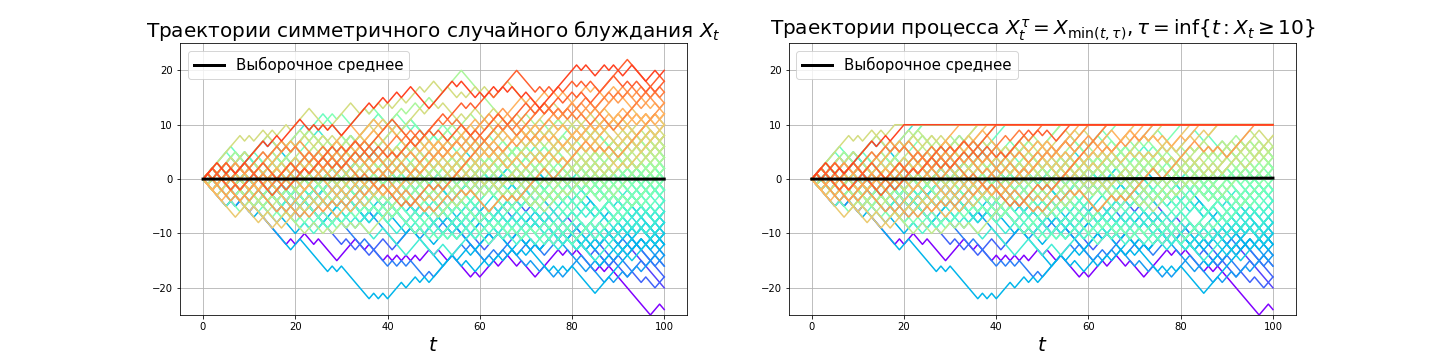
\includegraphics[width=1.0\textwidth]{1_figs/stopped_process.png}
    \end{center}

\end{frame}

\begin{frame}{Теорема Дуба об оптимальной остановке}
    \begin{block}{Теорема}
        Пусть $X_t$ -- мартингал, $\tau$ -- момент остановки. Пусть выполнено одно из условий:
        \begin{itemize}
            \item $\tau$ -- ограничено, т.е. $\exists c : \PP(\tau \leq c) = 1$
            \item $\E \tau < \infty$, $\exists c:  \; \forall t \; \E \left[ |X_{t+1}-X_t| \F_t\right] \leq c$
            \item $X_t^{\tau}$ равномерно ограничено, т.е. $\exists c : \forall t \; |X_t^{\tau}| \leq c$
        \end{itemize}
        Тогда $\E X_{\tau} = \E X_0$
    \end{block}
    \pause
    \textit{Доказательство}
    По предыдущей теореме $X_t^{\tau}$ -- мартингал, откуда $\E X_t^{\tau} = \E X_0$. Переходим к пределу при $t\to\infty$, получаем $$\E X_t^{\tau} = \E X_{\min(t, \tau)} \to \E X_{\tau}$$
    
    Условия теоремы нужны для обоснования сходимости.\qed
\end{frame}
\begin{frame}{Теорема Дуба о разложении}
\only<1>{
    \begin{block}{Теорема}
        Пусть $X_t$ -- согласованный интегрируемый процесс. Тогда $\exists! \; (M_t)_{t\geq 0}$ и $(A_t)_{t\geq 0}$ такие, что:
        \begin{itemize}
            \item $M_t$ -- мартингал,
            \item $A_t$ -- предсказуемый процесс и $A_0=0$
            \item $X_t = M_t + A_t$
        \end{itemize}
    \end{block}}
\only<2>{
    \textit{Доказательство}. Пусть такое разложение существует, тогда:
    $$
        \E [X_t |\F_{t-1}] = \E [M_t + A_t | F_{t-1}] = M_{t-1} + A_t
        = X_{t-1} + (A_t - A_{t-1})
    $$Положим:
    \begin{itemize}
        \item $A_0 = 0, \; A_t = A_{t-1} + \E [X_t |\F_{t-1}] - X_{t-1}$
        \item $M_t = X_t - A_t$
    \end{itemize}
    Очевидно, $A_t$ -- предсказуемый процесс, разложение $X_t=M_t+A_t$ выполнено автоматически, достаточно проверить мартингальность $M_t$:
    \begin{align*}
        &\E [M_t | \F_{t-1}] = \E [X_t | \F_{t-1}] - A_t 
        = \\
        &= \E [X_t | \F_{t-1}] - \left( A_{t-1} + \E [X_t |\F_{t-1}] - X_{t-1} \right) = \\
        &= X_{t-1}-A_{t-1}=M_{t-1}
    \end{align*}
    \qed}
\end{frame}

\begin{frame}{Теорема Дуба о разложении}
    \textit{Пример}. Пусть $X_t$ -- симметричное случайное блуждание, Тогда $X_t^2 = M_t + A_t$, где 
    \begin{itemize}
        \item $A_t = t$ -- предсказуемый процесс (детерминированный)
        \item $M_t = X_t^2 - t$ -- мартингал (докажите) 
    \end{itemize}
\end{frame}


\end{document}